\subsection{Motivation}
The autonomous vehicles (AVs) is the evolutionary direction of automobiles  due to its promising reliability and efficiency, as well as the underlying commercial profits. To gain a comprehensive perception of the driving environment is the very essential step for AVs. Object detection is one of the key challenges of perception. Thanks to the remarkable advancement of deep neural networks, great achievements have been made on 2D object detection, while 3D object detection is still underdeveloped. For example, according to the  KITTI Object Detection Benchmark\cite{Geiger2012CVPR}, the Average Precision (AP) of  top 10 2D car detection algorithms is over 90\% whereas best performance of 3D car detection is only 73.66\%. This gap results from the difficulty of adding the third dimension and the orientation of the 3D bounding box.

For AVs, 3D information of the surrounding vehicles is indispensable because it expresses the vehicle dimensions, locations and orientation in the real 3D environment, which is essential for AVs to perform planning and decision making. To find a safe and efficient route, the information of actual and potential movement, dimensions, and location of other vehicles is necessary. In order to perceive the movement, 3D localization,  orientation, and time are used to recover the velocity. The decision-making systems are more complicated and require more detailed 3D information, for example, the Bosch's Autonomous Emergency Braking systems (AEB) requires the distance to each part of a foregoing vehicle to decide whether or which level of brakes to apply.And it is common that some parts of the vehicle are occluded by other objects or truncated by the boundaries of the image. Thus, the exact location of each vehicle part and the visibility property of these parts are necessary.

Here we propose an approach that can simultaneously present the 3D dimensions, 3D localization, 3D bounding box orientation, 3D parts location, and parts visibility of a vehicle by giving a monocular image and all the 2D bounding boxes for vehicles. Figure 1 \tbd shows one output image example.

\begin{figure}[h]		
	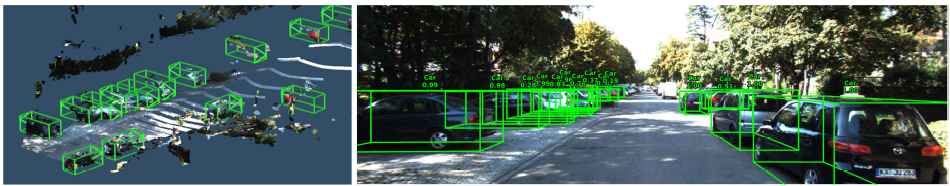
\includegraphics[width=1\textwidth]{bev_ex1.png}
	\caption{a}
	\centering
	\label{figure:a}
\end{figure}

